% Set the document class and theme
\documentclass{beamer}

\usetheme{Madrid}
\useoutertheme{miniframes} % Alternatively: miniframes, infolines, split
\useinnertheme{circles}

\definecolor{IITHorange}{RGB}{243, 130, 33} % UBC Blue (primary)
\definecolor{IITHyellow}{RGB}{254, 203, 10} % UBC Grey (secondary)

\setbeamercolor{palette primary}{bg=IITHorange,fg=white}
\setbeamercolor{palette secondary}{bg=IITHorange,fg=white}
\setbeamercolor{palette tertiary}{bg=IITHorange,fg=white}
\setbeamercolor{palette quaternary}{bg=IITHorange,fg=white}
\setbeamercolor{structure}{fg=IITHorange} % itemize, enumerate, etc
\setbeamercolor{section in toc}{fg=IITHorange} % TOC sections

% Override palette coloring with secondary
\setbeamercolor{subsection in head/foot}{bg=IITHyellow,fg=white}

\setbeamertemplate{caption}[numbered]
\setbeamertemplate{theorems}[numbered]

\usepackage{./presentation_macros}

\title[Cryptanalysis of DES]{CS5760: Cryptanalysis of DES and DES-like Iterated Cryptosystems}
\date{February 3, 2025}
\author{Gautam Singh}
\institute[IITH]{Indian Institute of Technology Hyderabad}

\begin{document}
	
	\begin{frame}
		\titlepage
	\end{frame}
	
	\begin{frame}
		\tableofcontents
	\end{frame}
	
	\section{Introduction}
	
	\begin{frame}
		\frametitle{Differential Cryptanalysis}
		\begin{columns}
			\begin{column}{0.65\textwidth}
				\begin{enumerate}
					\item<1-> Chosen plaintext attack.
					\item<1-> Exploit XOR between plaintext pairs to find key bits.
					\item<2-> Per DES round, XOR of respective inputs is:
					\begin{itemize}
						\item \emph{Linear} in expansion \(E\) to get \(S_E\).
						\item \emph{Invariant} in key mixing with subkey \(S_K\)
						to get \(S_I = S_E \oplus S_K\).
						\item \emph{Linear} in permutation \(P\) on \(S_O\)
						after S boxes.
						\item \emph{Invariant} in XOR operation connecting
						rounds.
					\end{itemize}
					\item<3-> S boxes are \emph{nonlinear}. Probability analysis
					performed between input and output XOR.
				\end{enumerate}
			\end{column}
			\begin{column}{0.35\textwidth}
				\begin{figure}[!ht]
					\centering
					\includegraphics<2->[width=\columnwidth]{images/des_f.png}
					\only<2->{\caption{\(F\) function of DES.}}
					\label{fig:des-f}
				\end{figure}
			\end{column}
		\end{columns}
	\end{frame}

	\section[S Boxes]{Probability Analysis of S Boxes}
	
	\begin{frame}
		\frametitle{Probability Analysis of S Boxes}
		\begin{enumerate}
			\item Suppose \(Si_I^\prime = Si_I \oplus Si_I^*\) is the input XOR
			to the \(i\)\textsuperscript{th} S box, and \(Si_O^\prime\) is the
			output XOR (\(1 \le i \le 8\)).
			\item<2-> We create a \emph{pairs XOR distribution table} for each S
			box.
			\begin{itemize}
				\item Each entry \(\brak{Si_I^\prime, Si_O^\prime}\) equals the
				number of 6-bit key blocks \(Si_K\) for which \(Si_I^\prime
				\rightarrow Si_O^\prime\).
				\item 64-by-16 joint probability mass function.
			\end{itemize}
			\item<3-> This joint PMF can reduce the number of possible
			(sub)keys. Used to drive choice for the plaintext XOR.
			\begin{itemize}
				\item \(\approx 80\%\) entries are non-zero/possible for each S
				box (some have lesser percentages).
				\item Given \(Si_I^\prime\) and \(Si_O^\prime\), we can narrow
				down \(Si_K\) to a few possibilities.
			\end{itemize}
			\item<4-> \(i\)\textsuperscript{th} S box contributes probability
			\(p_i\) for \(Si_I^\prime \rightarrow Si_O^\prime\). 
			\begin{itemize}
				\item For \(X \rightarrow Y\) over a round, \(P = \prod_i p_i\).
				\item Over \(n\) rounds, \(P = \prod_{i=1}^n P_i\).
			\end{itemize}
			\only<5->{\bfseries Desirable for cryptanalysis: high \(P\) with
			large \(n\).}
		\end{enumerate}
	\end{frame}

	\section{Characteristic}

	\begin{frame}
		\frametitle{Characteristic}
		Formalizes notion of high-probability plaintext XORs.
		\begin{definition}[Characteristic]
			An \emph{n-round chracteristic} is a tuple \(\Omega =
			\brak{\Omega_P, \Omega_\Lambda, \Omega_T}\) where \(\Omega_P =
			\brak{L^\prime, R^\prime}\) and \(\Omega_T = \brak{l^\prime,
			r^\prime}\) are \(m\) bit numbers, \(\Omega_\Lambda =
			\brak{\Lambda_1, \ldots, \Lambda_n}\), \(\Lambda_i =
			\brak{\lambda_I^i, \lambda_O^i}\) and \(\lambda_I^i,
			\lambda_O^i, L^\prime, R^\prime, l^\prime, r^\prime\) are
			\(\frac{m}{2}\) bit numbers and \(m\) is the block size of the
			cryptosystem satisfying
			\begin{align}
				\lambda_I^1 &= R^\prime \\
				\lambda_I^2 &= L^\prime \oplus \lambda_O^1 \\
				\lambda_I^n &= r^\prime \\
				\lambda_I^{n-1} &= l^\prime \oplus \lambda_O^n \\
				\forall\ 1 < i < n,\ \lambda_O^i &= \lambda_I^{i-1} \oplus \lambda_I^{i+1}
				\label{eq:char-def}
			\end{align}
		\end{definition}
	\end{frame}

	\begin{frame}
		\frametitle{Characteristic}
		\begin{definition}[Right Pair]
			A \emph{right pair with respect to an n-round characteristic
			\(\Omega = \brak{\Omega_P, \Omega_\Lambda, \Omega_T}\) and an
			independent key \(K\)} is a pair for which \(P^\prime = \Omega_P\)
			and for each round \(i\) of the first \(n\) rounds of the encryption
			of the pair using \(K\) the input XOR of the
			\(i\)\textsuperscript{th} round equals \(\lambda_I^i\) and the
			output XOR of the \(F\) function equals \(\lambda_O^i\). Pairs that
			do not satisfy these conditions are called \emph{wrong pairs}.
		\end{definition}
		\pause
		\begin{definition}[Probability of a Round of a Characteristic]
			Round \(i\) of an \(n\)-round characteristic \(\Omega\) has
			probability \(p_i^\Omega\) if \(\lambda_I^i \rightarrow
			\lambda_O^i\) with probability \(p_i^\Omega\) by the \(F\) function.
		\end{definition}
	\end{frame}

	\begin{frame}
		\frametitle{Probability of a Characteristic}
		\begin{definition}[Probability of a Characteristic]
			An \(n\)-round characteristic \(\Omega\) has probability
			\(p^\Omega\) given by
			\begin{equation}
				p^\Omega = \prod_{i=1}^n p_i^\Omega
				\label{eq:prob-char}
			\end{equation}
		\end{definition}
		\pause
		\begin{theorem}[Probability of a Characteristic and Right Pairs]
			The formally defined probability of a characteristic \(\Omega =
			\brak{\Omega_P, \Omega_\Lambda, \Omega_T}\) is the probability that
			any fixed plaintext pair satisfying \(P^\prime = \Omega_P\) is a
			right pair when random independent keys are used.
		\end{theorem}
		\pause
		\begin{proof}[Proof Idea]
			Keys \emph{randomize} the inputs to the S boxes in each round.
		\end{proof}
	\end{frame}

	\begin{frame}
		\frametitle{Example of a Characteristic}
		\begin{figure}[!ht]
			\centering
			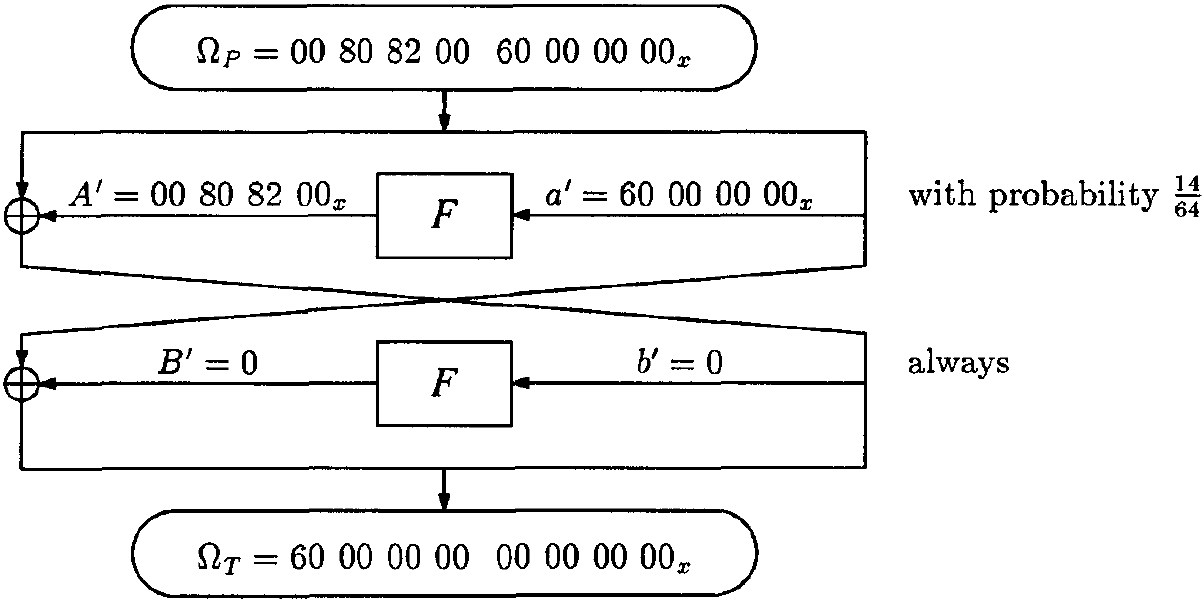
\includegraphics[width=0.9\linewidth]{images/des_char.png}
			\caption{Example of a two-round characteristic with probability \(\frac{14}{64}\).}
			\label{fig:des-char-example}
		\end{figure}
	\end{frame}

	\section{Signal to Noise Ratio}
	
	\begin{frame}
		\frametitle{Signal to Noise Ratio}
		\begin{enumerate}
			\item Right pairs will always suggest the right key value. But right
			pairs occur with probability \(p^\Omega\).
			\item<2-> On the other hand, wrong pairs suggest a randomly chosen
			key (not necessarily the right key in the worst case).
			\item<3-> Suitable counting approach on the key values will
			``spike'' at the right key and have smaller but approximately equal
			counts at other keys.
			\item<4-> The key with the largest count is likely the actual key.
		\end{enumerate}
		\begin{definition}<5->[Signal-to-Noise Ratio]
			The ratio between the number of right pairs and the average count of
			incorrect subkeys in a counting scheme is called the \emph{signal to
			noise ratio of the counting scheme} and is denoted by \(S/N\).
		\end{definition}
	\end{frame}

	\begin{frame}
		\frametitle{Computing the SNR}
		Consider the variables shown in \cref{tab:snr-vars}.
		\begin{table}[!ht]
			\centering
			\begin{tabular}{|c|l|}
				\hline
				\textbf{Variable} & \textbf{Definition} \\
				\hline
				\(p\) & Probability of the characteristic \\
				\hline
				\(m\) & Number of created pairs \\
				\hline
				\(\alpha\) & Average count per analyzed pair \\
				\hline
				\(\beta\) & Fraction of analyzed pairs \\
				\hline
				\(k\) & Number of key bits counted on \\
				\hline
			\end{tabular}
			\caption{Table of variables to compute the SNR.}
			\label{tab:snr-vars}
		\end{table}
		\pause
		Then,
		\begin{equation}
			S/N = \frac{m \cdot p}{\frac{m \cdot \beta \cdot \alpha}{2^k}} = \frac{2^k \cdot p}{\alpha \cdot \beta}
			\label{eq:snr-expr}
		\end{equation}
	\end{frame}

	\section{Structures}

	\begin{frame}
		\frametitle{Structures}
		\begin{enumerate}
			\item<1-> Many attacks on DES use more than one characteristic.
			\item<2-> Requirement to minimize the amount of plaintexts generated.
			\begin{definition}<3->[Quartet and Octet]
				A \emph{quartet} is a structure of four ciphertexts that
				simultaneously contains two ciphertext pairs of one
				characteristic and two ciphertext pairs of a second
				characteristic. An \emph{octet} is a structure of eight
				ciphertexts that simultaneously contains four ciphertext pairs
				of each of three characteristics.
			\end{definition}
			\item<3-> As an example, \(\brak{P, P \oplus \Omega_P^1, P \oplus
			\Omega_P^2, P \oplus \Omega_P^1 \oplus \Omega_P^2}\) is a quartet.
			\item<4-> Quartets save \(\frac{1}{2}\) of the data and octets save
			\(\frac{2}{3}\) of the data.
		\end{enumerate}
	\end{frame}

	\section[Cryptanalysis]{Differential Cryptanalysis of DES Variants}

	\subsection{DES Reduced to Four Rounds}

	\begin{frame}
		\frametitle{DES Reduced to Four Rounds}
		\begin{enumerate}
			\item<1-> Use two one-round characteristics, as shown in
			\cref{fig:des-4rd-char}.
			\item<2-> Both characteristics have probability 1.
			\item<3-> Example of a \emph{3R-attack}. There are \emph{three}
			extra rounds after the characteristic is applied.
		\end{enumerate}
		
		\visible<2->{
			\begin{figure}[!ht]
				\centering
				\begin{subfigure}[t]{0.4\linewidth}
					\centering
					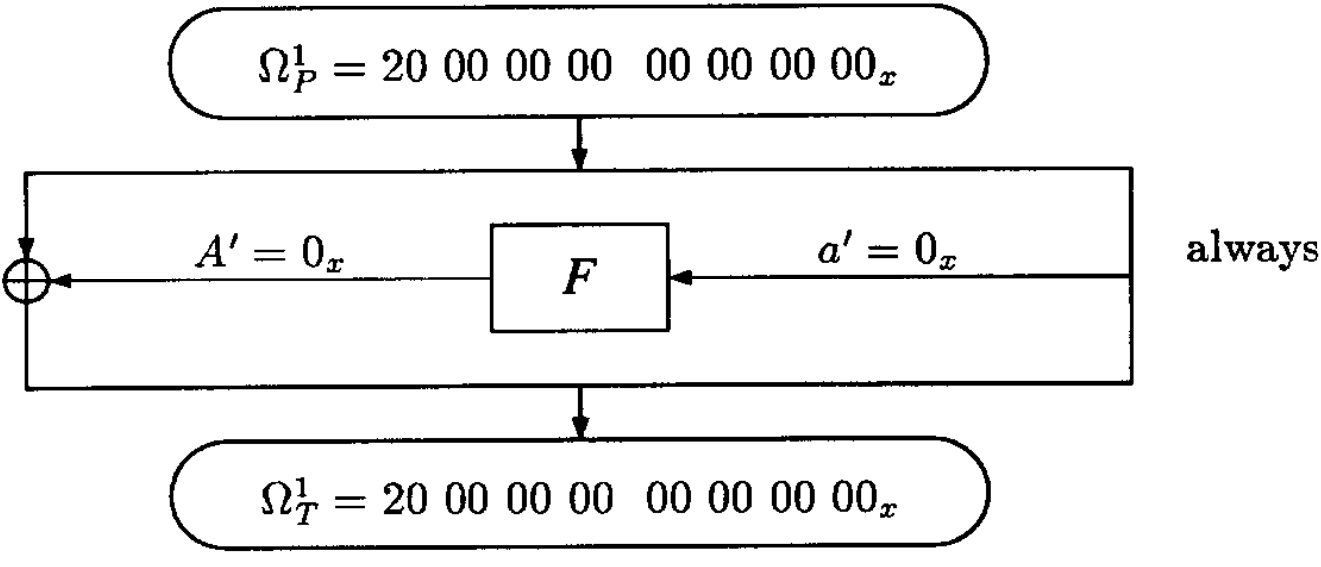
\includegraphics[width=\columnwidth]{images/des_4round_char.png}
				\end{subfigure}
				~
				\begin{subfigure}[t]{0.4\linewidth}
					\centering
					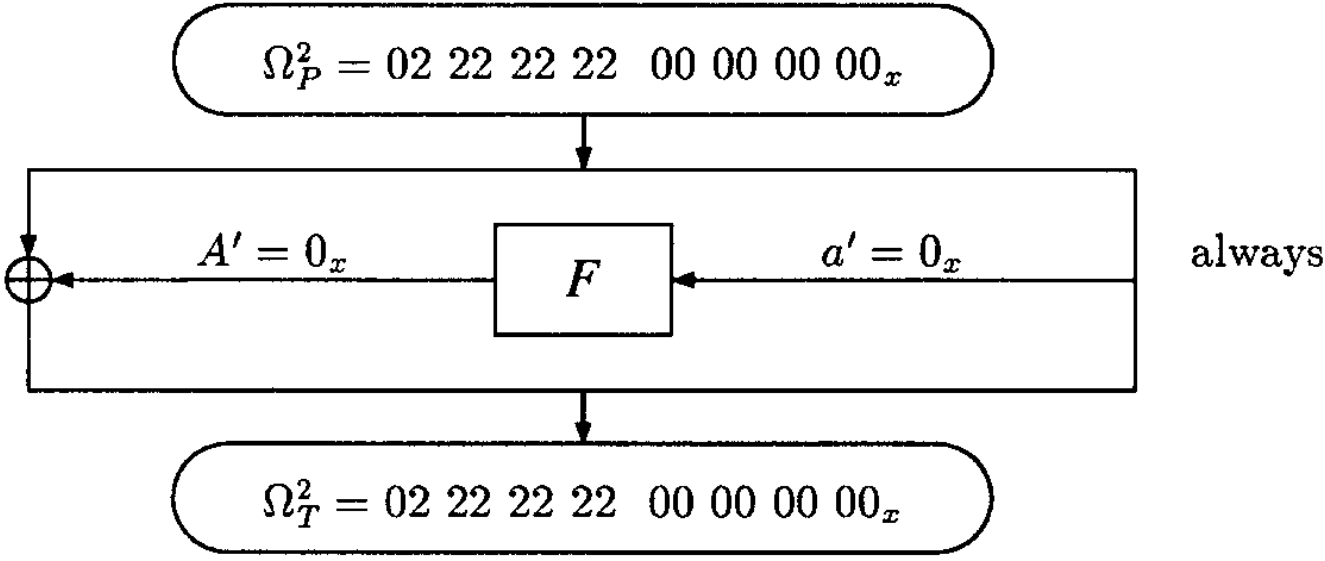
\includegraphics[width=\columnwidth]{images/des_4round_char2.png}
				\end{subfigure}
				\caption{Characteristics used for cryptanalysis of DES reduced to four rounds.}
				\label{fig:des-4rd-char}
			\end{figure}
		}
	\end{frame}

	\begin{frame}
		\frametitle{DES Reduced to Four Rounds}
		\begin{columns}
			\begin{column}{0.65\textwidth}
				\begin{enumerate}
					\item<2-> Using \(\Omega^1\), we have
					\begin{equation}
						c^\prime = D^\prime \oplus l^\prime = a^\prime \oplus B^\prime \implies D^\prime = B^\prime \oplus l^\prime
						\label{eq:des-4rd-D}
					\end{equation}
					\item<3-> We have \(a^\prime = 0_x \implies A^\prime = 0_x\)
					and \(b^\prime = A^\prime \oplus L^\prime = L^\prime\).
					\begin{itemize}
						\item<4-> In the second round S2, \dots, S8 receive
						zero XOR input.
						\item<5-> 28 bits of \(B^\prime\) are zero and hence we
						can find \emph{28 bits of \(D^\prime\)}.
						\item<6-> We already know \(d^\prime = r^\prime\). So,
						we employ a counting approach to get \(K4\).
					\end{itemize}
				\end{enumerate}
			\end{column}
			\begin{column}{0.35\textwidth}
				\begin{figure}[!ht]
					\centering
					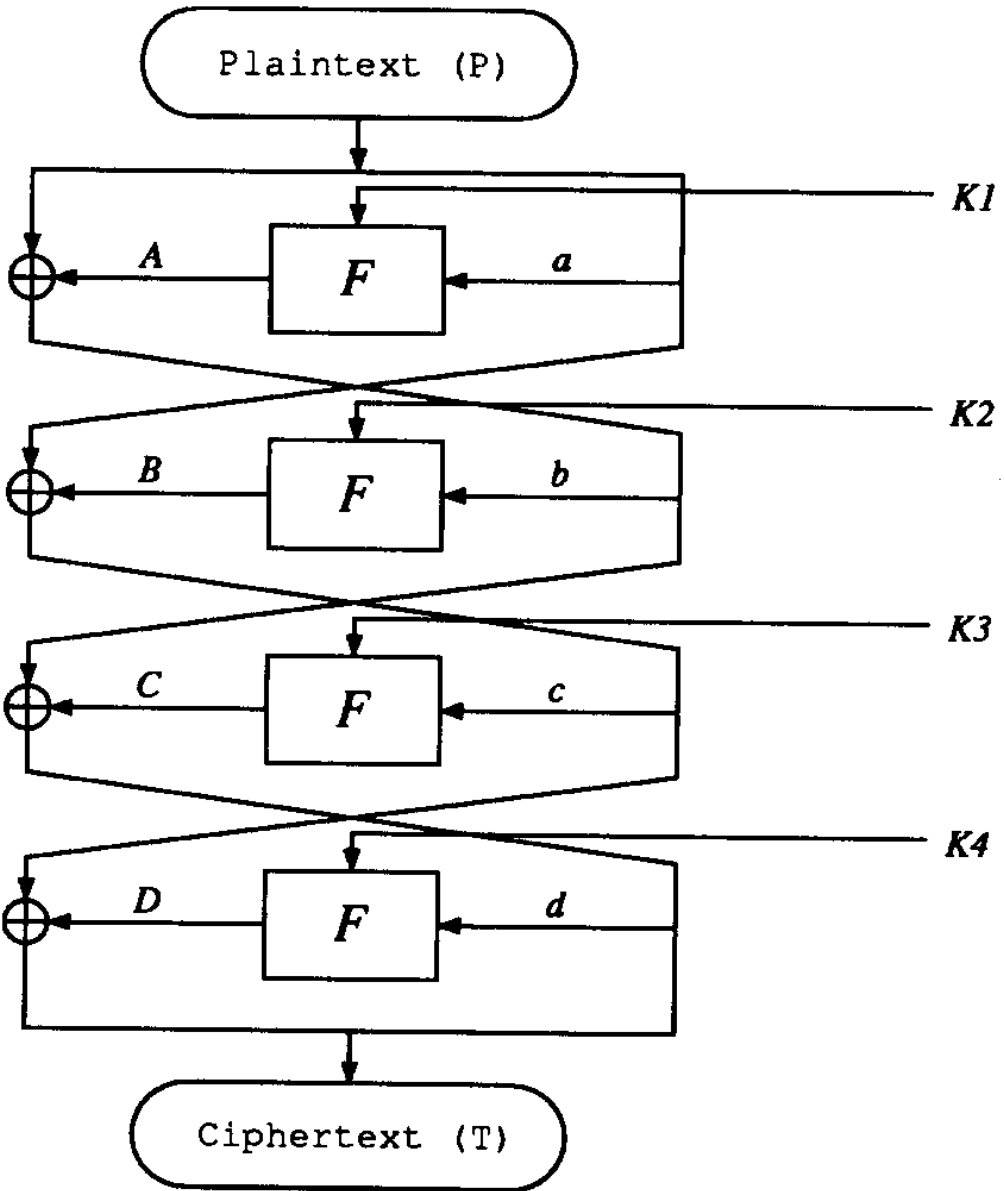
\includegraphics[width=\columnwidth]{images/des_4round.png}
					\caption{DES reduced to four rounds.}
					\label{fig:des-four}
				\end{figure}
			\end{column}
		\end{columns}
	\end{frame}

	\begin{frame}
		\frametitle{DES Reduced to Four Rounds}
		\begin{enumerate}
			\item<1-> To get \(Si_{Kd}\) for \(2 \le i \le 8\), we verify
			\eqref{eq:des-4rd-check}.
			\begin{equation}
				S\brak{S_{Ed} \oplus S_{Kd}} \oplus S\brak{S_{Ed}^* \oplus S_{Kd}} = S_{Od}^\prime
				\label{eq:des-4rd-check}
			\end{equation}
			\item Only \emph{one} plaintext pair is needed since characteristic
			probability is 1.
			\item We recover \(7 \times 6 = 42\) key bits of \(K4\), which
			correspond to 42 bits of the master key.
			\item Exhaustively search the other 14 key bits to get the entire
			master key.
			\item We have used the key schedule to our advantage here?
			\emph{What if all the keys were independent?}
		\end{enumerate}
	\end{frame}

	\begin{frame}
		\frametitle{DES Reduced to Four Rounds: Independent Subkeys}
		\begin{enumerate}
			\item<1-> We now use \(\Omega^2\) to get the remaining 6 subkey bits
			of \(K4\), as the input to S1 in the second round is now zero.
			\item<2-> We have \(C^\prime = b^\prime \oplus d^\prime\). Peeling
			off/decrypting one round will give us \(c^\prime\) completely.
			\begin{itemize}
				\item<3-> Since \(c^\prime\) and \(C^\prime\) are both
				completely known, \(K3\) can be completely found using a similar
				counting argument.
			\end{itemize}
			\item<4-> Since \(a^\prime = A^\prime = 0_x\), all keys are equally
			likely. Other characteristics \(\Omega^3\) and \(\Omega^4\) are
			chosen such that
			\begin{itemize}
				\item \(S_{Ea}^\prime \neq 0_x\) for all S boxes for both
				characteristics.
				\item For every S box, the \(S_{Ea}^\prime\) values differ
				between the characteristics.
				\item Similar counting methods used to get \(K1\) and \(K2\).
			\end{itemize}
			\item<5-> 16 chosen plaintexts are needed for this attack.
			\begin{itemize}
				\item 8 pairs of \(\Omega^1\) and \(\Omega^2\) each.
				\item 4 pairs of \(\Omega^3\) and \(\Omega^4\) each.
			\end{itemize}
			To reduce the data needed, two octets are used.
		\end{enumerate}
	\end{frame}

	\subsection{DES Reduced to Six Rounds}

	\begin{frame}
		\frametitle{<title>}
	
		
	
	\end{frame}
\end{document}